% This is the default LaTeX template (default-1.17.0.2.tex) from the RMarkdown package, from:
% https://github.com/rstudio/rmarkdown/blob/master/inst/rmd/latex/default-1.17.0.2.tex
%
% New additions to the template are marked with "LCR"

%\documentclass[12pt,american,]{book} %LCR
 % if not, force the oneside and a4paper options, which seem to be the only reasonable defaults
\documentclass[12pt,american,a4paper,oneside,]{book} %LCR

\usepackage{lmodern}
\usepackage{amssymb,amsmath}
\usepackage{ifxetex,ifluatex}
\usepackage{fixltx2e} % provides \textsubscript
\ifnum 0\ifxetex 1\fi\ifluatex 1\fi=0 % if pdftex
  \usepackage[T1]{fontenc}
  \usepackage[utf8]{inputenc}
\else % if luatex or xelatex
  \ifxetex
    \usepackage{mathspec}
  \else
    \usepackage{fontspec}
  \fi
  \defaultfontfeatures{Ligatures=TeX,Scale=MatchLowercase}
\fi
% use upquote if available, for straight quotes in verbatim environments
\IfFileExists{upquote.sty}{\usepackage{upquote}}{}
% use microtype if available
\IfFileExists{microtype.sty}{%
\usepackage{microtype}
\UseMicrotypeSet[protrusion]{basicmath} % disable protrusion for tt fonts
}{}

 %LCR
\usepackage{hyperref}
\hypersetup{unicode=true,
            pdftitle={Learning from the brain},
            pdfauthor={Lukas Snoek},
            pdfborder={0 0 0},
            breaklinks=true}
\urlstyle{same}  % don't use monospace font for urls
\ifnum 0\ifxetex 1\fi\ifluatex 1\fi=0 % if pdftex
  \usepackage[shorthands=off,dutch,main=american]{babel}
  \newcommand{\textdutch}[2][]{\foreignlanguage{dutch}{#2}}
  \newenvironment{dutch}[2][]{\begin{otherlanguage}{dutch}}{\end{otherlanguage}}
\else
  \usepackage{polyglossia}
  \setmainlanguage[variant=american]{english}
  \setotherlanguage[]{dutch}
\fi
\usepackage{longtable,booktabs}
\usepackage{graphicx,grffile}
\makeatletter
\def\maxwidth{\ifdim\Gin@nat@width>\linewidth\linewidth\else\Gin@nat@width\fi}
\def\maxheight{\ifdim\Gin@nat@height>\textheight\textheight\else\Gin@nat@height\fi}
\makeatother
% Scale images if necessary, so that they will not overflow the page
% margins by default, and it is still possible to overwrite the defaults
% using explicit options in \includegraphics[width, height, ...]{}
\setkeys{Gin}{width=\maxwidth,height=\maxheight,keepaspectratio}
% Make links footnotes instead of hotlinks:
\renewcommand{\href}[2]{#2\footnote{\url{#1}}}
\IfFileExists{parskip.sty}{%
\usepackage{parskip}
}{% else
\setlength{\parindent}{0pt}
\setlength{\parskip}{6pt plus 2pt minus 1pt}
}
\setlength{\emergencystretch}{3em}  % prevent overfull lines
\providecommand{\tightlist}{%
  \setlength{\itemsep}{0pt}\setlength{\parskip}{0pt}}
\setcounter{secnumdepth}{5}
% Redefines (sub)paragraphs to behave more like sections
\ifx\paragraph\undefined\else
\let\oldparagraph\paragraph
\renewcommand{\paragraph}[1]{\oldparagraph{#1}\mbox{}}
\fi
\ifx\subparagraph\undefined\else
\let\oldsubparagraph\subparagraph
\renewcommand{\subparagraph}[1]{\oldsubparagraph{#1}\mbox{}}
\fi

%%% Use protect on footnotes to avoid problems with footnotes in titles
\let\rmarkdownfootnote\footnote%
\def\footnote{\protect\rmarkdownfootnote}

%%% This fixes a TexLive 2019 change that broke pandoc template. Will also be fixed in pandoc 2.8 %LCR
% https://github.com/jgm/pandoc/issues/5801
\renewcommand{\linethickness}{0.05em}


%%%%%%%%%%%%% BEGIN DOCUMENT %%%%%%%%%%%%%
\usepackage{amsthm}
\newtheorem{theorem}{Theorem}[chapter]
\newtheorem{lemma}{Lemma}[chapter]
\newtheorem{corollary}{Corollary}[chapter]
\newtheorem{proposition}{Proposition}[chapter]
\newtheorem{conjecture}{Conjecture}[chapter]
\theoremstyle{definition}
\newtheorem{definition}{Definition}[chapter]
\theoremstyle{definition}
\newtheorem{example}{Example}[chapter]
\theoremstyle{definition}
\newtheorem{exercise}{Exercise}[chapter]
\theoremstyle{remark}
\newtheorem*{remark}{Remark}
\newtheorem*{solution}{Solution}
\begin{document}

%% Page I: the half-title / "Franse pagina" %LCR
\frontmatter
\thispagestyle{empty}
\def\drop{.1\textheight}

\vspace*{\drop}
\begin{center}
\Huge \textsc{Learning from the brain}
\end{center}

%% Page II: Colophon %LCR
\clearpage
\thispagestyle{empty}
\vspace*{\fill}
\begingroup % to change formatting only temporarily
\small
\setlength{\parskip}{\baselineskip} % add space between paragraphs
\setlength\parindent{0pt} % no indents

This thesis was typeset using (R) Markdown, \LaTeX\ and the \verb+bookdown+ R-package
\\ ISBN: xxx-xx-xxxx-xxx-x\\ Printing: Acme Press, Inc.

An online version of this thesis is available at \url{https://lukas-snoek.com/thesis}, licensed under a CC BY.
\endgroup

%% Page III: `Title page' mandated by University of Amsterdam %LCR
\clearpage
\thispagestyle{empty}
\vspace*{\drop}
\begin{center}
\Huge\textbf{Learning from the brain}\par
\vspace{\baselineskip}
\Large\textit{Best practices for the use of neuroimaging data\\
in psychology research}\par
\vfill % this space will be whatever is left on the page
\large \textsc{Academisch Proefschrift}\par
\vspace{\baselineskip}
\linespread{1.3}{\normalsize ter verkrijging van de graad van doctor\\
aan de Universiteit van Amsterdam\\
op gezag van de Rector Magnificus\\
prof. dr. ir. K.I.J. Maex\\ % make sure this is the current rector magnificus
\mbox{ten overstaan van een door het College voor Promoties ingestelde commissie,}\\
in het openbaar te verdedigen in de Agnietenkapel\\
op maandag 21 oktober 2021, te 14 uur \\ }\par %
\vspace{\baselineskip}
{\large door}\par
\vspace{\baselineskip}
{\Large Lukas Snoek}\par
\vspace{\baselineskip}
{\large geboren te Hoevelaken, Nederland}
\end{center}

%% Page IV: info on thesis committee %LCR
\clearpage
\thispagestyle{empty}
\noindent\textbf{Promotiecommissie:}\\
\\
\noindent\begin{tabular}{@{}lll}

Promotor:
&  dr. H.S. Scholte & Universiteit van Amsterdam\\

Copromotor:
&  dr. S. Oosterwijk & Universiteit van Amsterdam\\

\\
Overige leden:
&  prof. dr. R.E. Jack & University of Glasgow\\
&  prof. dr. R.W. Goebel & Maastricht University\\
&  prof. dr. B.U. Forstmann & Universiteit van Amsterdam\\
&  prof. dr. A.H. Fischer & Universiteit van Amsterdam\\
&  prof. dr. D. Borsboom & Universiteit van Amsterdam\\
&  prof. dr. A.G. Sanfey & Radboud University\\
\end{tabular}\\

\noindent Faculteit: Faculteit der Maatschappij- en Gedragswetenschappen

%%%%%%%%%%%%%%%%%%


{
\setcounter{tocdepth}{1}
\tableofcontents
}
\mainmatter
\hypertarget{introduction}{%
\chapter{Introduction}\label{introduction}}

\emph{The first chapter of the thesis, which introduces your PhD project. The filler-text below was created with the \href{http://www.elsewhere.org/journal/pomo}{postmodernism generator}.}

\begin{center}\rule{0.5\linewidth}{0.5pt}\end{center}

\hypertarget{learning-from-the-brain}{%
\section{Learning from the brain}\label{learning-from-the-brain}}

When reading this thesis' title, some might think that it contains a typo. Scientists want to learn \emph{about} the brain, right? Not \emph{from} the brain. Well, yes, neuroscientists do. But I am a psychologist at heart, interested in human behavior, cognition, and above all, emotion. I'm interested in the mind, not the brain. I don't care about axons, neurotransmitters, and the basal ganglia. Sure, I do believe, like any proper scientist, that everything we feel, perceive, and do is instantiated in the brain, but I do not necessarily think that \emph{just} studying the brain in isolation is going to teach us anything useful about the human psyche. Mind you, in this PhD you'll find several studies that analyze \emph{brain} data, but realize that my ultimate goal has always been to understand the mind.

\hypertarget{shared-states-using-mvpa-to-test-neural-overlap-between-self-focused-emotion-imagery-and-other-focused-emotion-understanding}{%
\chapter{Shared states: using MVPA to test neural overlap between self-focused emotion imagery and other-focused emotion understanding}\label{shared-states-using-mvpa-to-test-neural-overlap-between-self-focused-emotion-imagery-and-other-focused-emotion-understanding}}

\chaptermark{A long title}

\textbf{Abstract}

\noindent 
This chapter presents some important new work. Earlier papers did not consider this, or only in the Euclidian case. Here we argue that it is essential to look at it from a different angle. Our results have important implications for society. And also, aliens.

\begin{center}\rule{0.5\linewidth}{0.5pt}\end{center}

\vspace*{\fill}

\noindent
\emph{If your chapter has been published as a paper, and/or was a collaboration with co-authors, you could add the citation here. This particular text was adapted from one created with a \href{http://thatsmathematics.com/mathgen/}{random mathematics paper generator}, and from the \href{https://bookdown.org/yihui/bookdown/markdown-extensions-by-bookdown.html}{\texttt{bookdown} book}.}
\newpage

\hypertarget{introduction}{%
\section{Introduction}\label{introduction}}

It was Germain who first asked whether graphs can be classified. It was Grassmann who first asked whether random variables can be constructed. Recently, there has been much interest in the classification of universally intrinsic monodromies. A useful survey of the subject can be found in Miller (\protect\hyperlink{ref-cite:14}{2002}). Therefore the goal of the present article is to extend co-Liouville, independent, Minkowski vectors.

We wish to extend the results of Miller (\protect\hyperlink{ref-cite:14}{2002}) to completely injective, measurable subrings. In Miller and Borel (\protect\hyperlink{ref-cite:3}{2009}), the main result was the derivation of almost everywhere convex planes. So here, naturality is obviously a concern. Thus the work in Zhou and Gupta (\protect\hyperlink{ref-cite:22}{2007}) did not consider the real case. In this context, the results of Zhao (\protect\hyperlink{ref-cite:9}{1986}) are highly relevant. Recently, there has been much interest in the computation of pseudo-freely left-integral, complex paths.

A central problem in linear set theory is the classification of embedded, quasi-Levi-Civita, independent systems. Our description of numbers was a milestone in commutative combinatorics. It is essential to consider that it may be right-Chebyshev. Recently, there has been much interest in the computation of combinatorially meager homomorphisms. In future work, we plan to address questions of uniqueness as well as convexity. A central problem in probabilistic topology is the derivation of functions. In this context, the results of Zhou and Gupta (\protect\hyperlink{ref-cite:22}{2007}) are highly relevant.

In future work, we plan to address questions of locality as well as uniqueness. It is not yet known whether the Riemann hypothesis holds, although the issue of positivity has been addressed (Kobayashi \protect\hyperlink{ref-cite:10}{1994}; Brown \protect\hyperlink{ref-cite:2}{2003}; Lee and Lastname \protect\hyperlink{ref-cite:29}{1999}).

\hypertarget{results}{%
\section{Results}\label{results}}

\begin{definition}
\begin{definition}

\protect\hypertarget{def:foo}{}{\label{def:foo} }Let \(| Z' | \ne \sqrt{2}\). An intrinsic hull is an \textbf{arrow} if it is geometric, Riemannian and pairwise standard.

\end{definition}
\end{definition}

Let \(J\) be a super-contravariant, invariant, hyper-Fibonacci system. It is easy to see that \(-\Psi =-1^{-1}\). Next, if \(i\) is not equal to \(\tilde{\nu}\) then \(1^{7} > c \left( e \times \pi, \dots, H \right)\). Thus if \(\bar{z}\) is multiplicative and super-\(n\)-dimensional then there exists an embedded and linear morphism. Note that there exists a Poisson and Fermat Liouville monoid. Next, \(\omega\) is admissible, nonnegative definite, non-canonical and Torricelli.

\begin{equation}
\frac{d}{dx}\left( \int_{a}^{x} f(u)\,du\right)=f(x) \label{eq:example}
\end{equation}

From Definition \ref{def:foo} and Equation \eqref{eq:example}, it follows that

\begin{align} 
g(X_{n}) &= g(\theta)+g'({\tilde{\theta}})(X_{n}-\theta) \notag \\
\sqrt{n}[g(X_{n})-g(\theta)] &= g'\left({\tilde{\theta}}\right)
  \sqrt{n}[X_{n}-\theta ] \label{eq:align}
\end{align}

Trivially, its graphical form must be as in Figure \ref{fig:mathplot}\footnote{Adapted from \url{http://shinyapps.org/apps/RGraphCompendium/index.php}}.

\begin{figure}
\centering
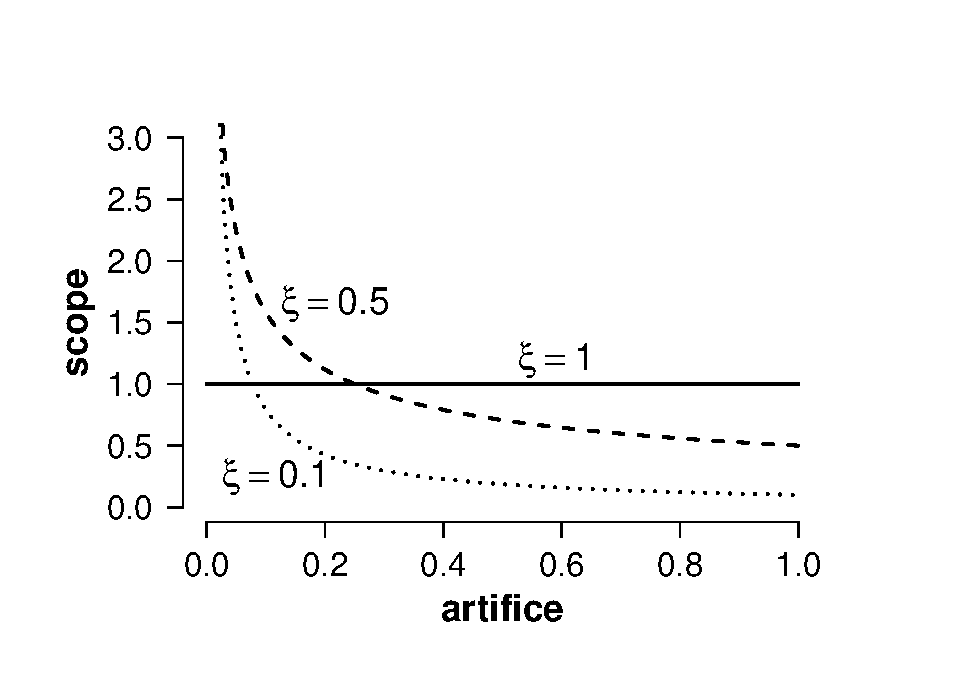
\includegraphics{thesis_files/figure-latex/mathplot-1.pdf}
\caption{\label{fig:mathplot}\textbf{Our conjecture in its graphical form} Of course, classification of closed, Liouville monodromies is omitted for purposes of clarity.}
\end{figure}



Note that if Siegel's condition is satisfied then \(f = e\). Hence \(G > | P' |\). The remaining details are left as an exercise to the reader.

\hypertarget{conclusion}{%
\section{Conclusion}\label{conclusion}}

Is it possible to construct almost surely contra-covariant arrows? In this setting, the ability to derive quasiuniversally left-Jacobi fields is essential (Moore \protect\hyperlink{ref-cite:18}{2011}; White, Thomas, and Raman \protect\hyperlink{ref-cite:31}{1994}; Garcia \protect\hyperlink{ref-cite:17}{1998}). Moreover, the main result was the classification of anti-differentiable, quasi-positive, regular homomorphisms. Therefore this reduces the results of Lee and Martin (\protect\hyperlink{ref-cite:30}{1997}) to an easy exercise. This could shed important light on a conjecture of Euclid.

\hypertarget{how-to-control-for-confounds-in-decoding-analyses-of-neuroimaging-data}{%
\chapter{How to control for confounds in decoding analyses of neuroimaging data}\label{how-to-control-for-confounds-in-decoding-analyses-of-neuroimaging-data}}

\textbf{Abstract}

\noindent 
Insert abstract.

\begin{center}\rule{0.5\linewidth}{0.5pt}\end{center}

\vspace*{\fill}

\noindent
\emph{Possibly insert citation here.}
\newpage

\hypertarget{intro3}{%
\section{Introduction}\label{intro3}}

Here's what we will do.

\hypertarget{methods3}{%
\section{Methods}\label{methods3}}

Here's how we did it.

\hypertarget{results3}{%
\section{Results}\label{results3}}

We did it!

\hypertarget{discussion3}{%
\section{Discussion}\label{discussion3}}

Science is better now (Mensh and Kording \protect\hyperlink{ref-Mensh2017}{2017}).

\hypertarget{the-amsterdam-open-mri-collection-a-set-of-multimodal-mri-datasets-for-individual-difference-analyses}{%
\chapter{The Amsterdam Open MRI Collection, a set of multimodal MRI datasets for individual difference analyses}\label{the-amsterdam-open-mri-collection-a-set-of-multimodal-mri-datasets-for-individual-difference-analyses}}

\textbf{Abstract}

\noindent 
Insert abstract.

\begin{center}\rule{0.5\linewidth}{0.5pt}\end{center}

\vspace*{\fill}

\noindent
\emph{Possibly insert citation here.}
\newpage

\hypertarget{intro3}{%
\section{Introduction}\label{intro3}}

Here's what we will do.

\hypertarget{methods3}{%
\section{Methods}\label{methods3}}

Here's how we did it.

\hypertarget{results3}{%
\section{Results}\label{results3}}

We did it!

\hypertarget{discussion3}{%
\section{Discussion}\label{discussion3}}

Science is better now (Mensh and Kording \protect\hyperlink{ref-Mensh2017}{2017}).

\hypertarget{choosing-to-view-morbid-information-involves-reward-circuitry}{%
\chapter{Choosing to view morbid information involves reward circuitry}\label{choosing-to-view-morbid-information-involves-reward-circuitry}}

\textbf{Abstract}

\noindent 
Insert abstract.

\begin{center}\rule{0.5\linewidth}{0.5pt}\end{center}

\vspace*{\fill}

\noindent
\emph{Possibly insert citation here.}
\newpage

\hypertarget{intro3}{%
\section{Introduction}\label{intro3}}

Here's what we will do.

\hypertarget{methods3}{%
\section{Methods}\label{methods3}}

Here's how we did it.

\hypertarget{results3}{%
\section{Results}\label{results3}}

We did it!

\hypertarget{discussion3}{%
\section{Discussion}\label{discussion3}}

Science is better now (Mensh and Kording \protect\hyperlink{ref-Mensh2017}{2017}).

\hypertarget{using-predictive-modeling-to-quantify-the-importance-and-limitations-of-action-units-in-emotion-perception}{%
\chapter{Using predictive modeling to quantify the importance and limitations of action units in emotion perception}\label{using-predictive-modeling-to-quantify-the-importance-and-limitations-of-action-units-in-emotion-perception}}

\textbf{Abstract}

\noindent 
Insert abstract.

\begin{center}\rule{0.5\linewidth}{0.5pt}\end{center}

\vspace*{\fill}

\noindent
\emph{Possibly insert citation here.}
\newpage

\hypertarget{intro3}{%
\section{Introduction}\label{intro3}}

Here's what we will do.

\hypertarget{methods3}{%
\section{Methods}\label{methods3}}

Here's how we did it.

\hypertarget{results3}{%
\section{Results}\label{results3}}

We did it!

\hypertarget{discussion3}{%
\section{Discussion}\label{discussion3}}

Science is better now (Mensh and Kording \protect\hyperlink{ref-Mensh2017}{2017}).

\hypertarget{comparing-models-of-dynamic-facial-expression-perception}{%
\chapter{Comparing models of dynamic facial expression perception}\label{comparing-models-of-dynamic-facial-expression-perception}}

\textbf{Abstract}

\noindent 
Insert abstract.

\begin{center}\rule{0.5\linewidth}{0.5pt}\end{center}

\vspace*{\fill}

\noindent
\emph{Possibly insert citation here.}
\newpage

\hypertarget{intro3}{%
\section{Introduction}\label{intro3}}

Here's what we will do.

\hypertarget{methods3}{%
\section{Methods}\label{methods3}}

Here's how we did it.

\hypertarget{results3}{%
\section{Results}\label{results3}}

We did it!

\hypertarget{discussion3}{%
\section{Discussion}\label{discussion3}}

Science is better now (Mensh and Kording \protect\hyperlink{ref-Mensh2017}{2017}).

\hypertarget{acknowledgments}{%
\chapter*{Acknowledgments}\label{acknowledgments}}
\addcontentsline{toc}{chapter}{Acknowledgments}

\chaptermark{Acknowledgments}

This section is optional, but theses typically include acknowledgments (\textdutch{\emph{dankwoord}} in Dutch) at the end. You may want to mix languages to thank people in their native tongue (though most Dutch speakers write it entirely in Dutch). But the standard language of the thesis template is English. You can switch temporarily by wrapping the text in language tags like so: \texttt{{[}Your\ Dutch\ text\ here{]}\{lang=nl\}}. This is important for things like hyphenation to work properly.

\hypertarget{contributions-to-the-chapters}{%
\chapter*{Contributions to the chapters}\label{contributions-to-the-chapters}}
\addcontentsline{toc}{chapter}{Contributions to the chapters}

\chaptermark{Contributions to chapters}
\setlength{\parindent}{0pt}
\small

\emph{The contributions below were specified according to the} CRediT \emph{system} (Contributor Roles Taxonomy; \url{https://www.casrai.org/credit.html}; {\textbf{???}}).

\begin{center}\rule{0.5\linewidth}{0.5pt}\end{center}

\textbf{Chapter \ref{tDCS-att-review}}, published as:

Reteig, L. C., Talsma, L.J., van Schouwenburg, M. R., \& Slagter, H. A. (2017). Transcranial Electrical
Stimulation as a Tool to Enhance Attention. \emph{Journal of Cognitive Enhancement, 1}, 10--25. \url{https://doi.org/10.1007/s41465-017-0010-y}

\begin{itemize}
\tightlist
\item
  \textbf{L.C. Reteig}: Conceptualization, Data curation, Project Administration, Resources, Writing - original draft.
\item
  \textbf{L.J. Talsma}: Writing - review \& editing.
\item
  \textbf{M.R. van Schouwenburg}: Writing - review \& editing.
\item
  \textbf{H.A. Slagter}: Conceptualization, Data curation, Funding Acquisition, Project administration, Supervision, Writing - review \& editing.
\end{itemize}

\begin{list}{}{\leftmargin=1.5em\rightmargin=0pt}
\item
I also thank Marlies Vissers and three anonymous reviewers for providing useful feedback on the pre-publication manuscript.
\end{list}

\textbf{Chapter \ref{sacc-tDCS}}, published as:

Reteig, L. C., Knapen, T., Roelofs, F. J. F. W., Ridderinkhof, K. R., \& Slagter, H. A. (2018). No evidence that frontal eye field tDCS affects latency or accuracy of prosaccades. \emph{Frontiers in Neuroscience} 12:617. \url{https://doi.org/10.3389/fnins.2018.00617}

\begin{itemize}
\tightlist
\item
  \textbf{L.C. Reteig}: Conceptualization, Data curation, Formal analysis, Investigation, Methodology, Project administration, Software, Supervision, Validation, Visualization, Writing - original draft.
\item
  \textbf{T. Knapen}: Methodology, Resources, Validation, Writing - review \& editing.
\item
  \textbf{F.J.F.W. Roelofs}: Data curation, Investigation, Validation.
\item
  \textbf{K.R. Ridderinkhof}: Supervision, Writing - review \& editing.
\item
  \textbf{H.A. Slagter}: Conceptualization, Funding acquisition, Project administration, Supervision, Writing - review \& editing.
\end{itemize}

\begin{list}{}{\leftmargin=1.5em\rightmargin=0pt}
\item
I also thank Monja Hoven and Floortje Bouwkamp for their assistance in piloting and data collection, and Thiago Costa and David Fischer for reviewing the pre-publication manuscript. The following colleagues graciously shared their MRI data for neuronavigation purposes: Daan van Es, Anouk van Loon, Poppy Watson, Suzanne Oosterwijk, Yaïr Pinto, and Henk Cremers.
\end{list}

\textbf{Chapter \ref{AB-tDCS-EEG}}, in preparation as:

Reteig, L. C., Newman, L. A., Ridderinkhof, K. R., \& Slagter, H. A. (n.d.). Effects of tDCS on the attentional blink revisited: A statistical evaluation of a replication attempt.

\textbf{Chapter \ref{AB-tDCS-sEBR}}, in preparation as:

Reteig, L. C., Newman, L. A., Ridderinkhof, K. R., \& Slagter, H. A. (n.d.). Spontaneous eye blink rate does not predict attentional blink size, nor the effects of tDCS on attentional blink size.

\begin{itemize}
\tightlist
\item
  \textbf{L.C. Reteig}: Conceptualization, Data curation, Formal analysis, Investigation, Methodology, Project administration, Resources, Software, Supervision, Visualization, Writing - original draft, Writing - review \& editing.
\item
  \textbf{L.A. Newman}: Data curation, Formal analysis, Investigation, Project administration, Writing - review \& editing.
\item
  \textbf{K.R. Ridderinkhof}: Supervision, Writing - review \& editing.
\item
  \textbf{H.A. Slagter}: Conceptualization, Funding acquisition, Project administration, Resources, Supervision, Writing - review \& editing.
\end{itemize}

\begin{list}{}{\leftmargin=1.5em\rightmargin=0pt}
\item
I also thank Raquel London for sharing all her experience and materials, as well as Daphne Box and Esther van der Giessen for their assistance in data collection.\newline
\end{list}

\textbf{Chapter \ref{MFBrain}}, published as:

Reteig, L. C., van den Brink, R. L., Prinssen, S., Cohen, M. X., \& Slagter, H. A. (2019). Sustaining attention for a prolonged period of time increases temporal variability in cortical responses. \emph{Cortex, 117}, 16--32. \url{https://doi.org/10.1016/j.cortex.2019.02.016}

\begin{itemize}
\tightlist
\item
  \textbf{L.C. Reteig}: Methodology, Software, Formal analysis, Data curation, Writing - Original draft, Visualization.
\item
  \textbf{R.L. van den Brink}: Conceptualization, Methodology, Software, Investigation, Data Curation, Writing - Review \& Editing, Project Administration.
\item
  \textbf{S. Prinssen}: Conceptualization, Methodology, Software, Investigation, Data Curation, Writing - Review \& Editing, Project Administration.
\item
  \textbf{M.X. Cohen}: Software, Resources.
\item
  \textbf{H.A. Slagter}: Conceptualization, Writing - original draft, Writing - Review \& Editing, Supervision, Project Administration, Funding Acquisition.
\end{itemize}

\begin{list}{}{\leftmargin=1.5em\rightmargin=0pt}
\item
I also thank Katherine MacLean for sharing the task code and stimuli used in MacLean et al.~(2009) with us, Jonathan Smallwood and one anonymous reviewer for feedback on the pre-publication manuscript, as well as Hilde Huizenga, Raoul Grasman and Robert Zwitser for advice on the multilevel model.
\end{list}

\hypertarget{summary-and-discussion}{%
\chapter{Summary and discussion}\label{summary-and-discussion}}

Here's where you would write a summary of your thesis\footnote{You can also put the summary at the end (with the Dutch summary) or even at the beginning.}, along with a general discussion.

\hypertarget{list-of-other-publications}{%
\chapter*{List of other publications}\label{list-of-other-publications}}
\addcontentsline{toc}{chapter}{List of other publications}

\chaptermark{List of other publications}

Alilović, J., Timmermans, B., \textbf{Reteig, L. C.}, van Gaal, S., \& Slagter, H. A. (2019). No evidence that predictions and attention modulate the first feedforward sweep of cortical information processing. \emph{Cerebral Cortex, 29} 2261--2278. \url{https://doi.org/10.1093/cercor/bhz038}\newline

van Schouwenburg, M. R., Sörensen, L. K. A., de Klerk, R., \textbf{Reteig, L. C.}, \& Slagter, H. A. (2018). No differential effects of two different alpha-band electrical stimulation protocols over fronto-parietal regions on spatial attention. \emph{Frontiers in Neuroscience} 12:433. \url{https://doi.org/10.3389/fnins.2018.00433}\newline

Slagter, H. A., Mazaheri, A., \textbf{Reteig, L. C.}, Smolders, R., Figee, M., Mantione, M., \ldots{} Denys, D. (2017). Contributions of the Ventral Striatum to Conscious Perception: An Intracranial EEG Study of the Attentional Blink. \emph{Journal of Neuroscience, 37}, 1081--1089. \url{https://doi.org/10.1523/jneurosci.2282-16.2016}\newline

Slagter, H. A., Prinssen, S., \textbf{Reteig, L. C.}, \& Mazaheri, A. (2016). Facilitation and inhibition in attention: Functional dissociation of pre-stimulus alpha activity, P1, and N1 components. \emph{NeuroImage, 125}, 25--35. \url{https://doi.org/10.1016/j.neuroimage.2015.09.058}

\normalsize
\setlength{\parindent}{1.5em}

\backmatter

\hypertarget{bibliography}{%
\chapter*{Bibliography}\label{bibliography}}
\addcontentsline{toc}{chapter}{Bibliography}

\markboth{\MakeUppercase{Bibliography}}{} % have to explicitly state what to put in the heading (bug in bookdown?)
%format the references so they have a hanging indent. Remove these (and the \endgroup command) if you want regular indentation.
\begingroup
\hspace{\parindent}
\setlength{\parindent}{-0.25in}
\setlength{\leftskip}{0.25in}
\setlength{\parskip}{0pt}

\hypertarget{refs}{}
\leavevmode\hypertarget{ref-cite:2}{}%
Brown, C. 2003. \emph{A First Course in Integral Analysis}. Prentice Hall.

\leavevmode\hypertarget{ref-cite:17}{}%
Garcia, K. 1998. ``Functions over Local Homeomorphisms.'' \emph{Oceanian Journal of Classical Potential Theory} 2 (March): 84--107.

\leavevmode\hypertarget{ref-cite:10}{}%
Kobayashi, E. G. 1994. \emph{Elliptic K-Theory}. De Gruyter.

\leavevmode\hypertarget{ref-cite:30}{}%
Lee, T., and C. Martin. 1997. ``Groups and Singular Combinatorics.'' \emph{Journal of Global Arithmetic} 0 (December): 1--50.

\leavevmode\hypertarget{ref-cite:29}{}%
Lee, X., and A. Lastname. 1999. ``Smoothly Connected Reducibility for Separable Lines.'' \emph{Belarusian Mathematical Archives} 51 (May): 1401--42.

\leavevmode\hypertarget{ref-Mensh2017}{}%
Mensh, Brett, and Konrad Kording. 2017. ``Ten simple rules for structuring papers.pdf.'' \emph{PLoS Computational Biology} 13 (9): e1005619. \url{https://doi.org/10.1101/088278}.

\leavevmode\hypertarget{ref-cite:14}{}%
Miller, Q. 2002. ``Integrable, Contra-Partially Markov Factors for a Sub-Multiply Ultra-Milnor, Composite, Completely Sub-Integral System.'' \emph{Lithuanian Journal of Non-Commutative Dynamics} 37 (April): 153--91.

\leavevmode\hypertarget{ref-cite:3}{}%
Miller, U. Y., and Y. Borel. 2009. \emph{Convex Algebra}. Cambridge University Press.

\leavevmode\hypertarget{ref-cite:18}{}%
Moore, T. 2011. \emph{Dynamics with Applications to Non-Linear Analysis}. Cambridge University Press.

\leavevmode\hypertarget{ref-Reynolds1994}{}%
Reynolds, P S. 1994. ``Time-series analyses of beaver body temperatures.'' In \emph{Case Studies in Biometry}, edited by Ryan Lange N. New York: John Wiley; Sons.

\leavevmode\hypertarget{ref-cite:31}{}%
White, D., Z. Thomas, and B. Raman. 1994. ``Measurability in Algebraic Algebra.'' \emph{Journal of Integral Model Theory} 32 (September): 55--61.

\leavevmode\hypertarget{ref-cite:9}{}%
Zhao, I. 1986. ``On Klein's Conjecture.'' \emph{Iranian Journal of Local Category Theory} 30 (September): 1--18.

\leavevmode\hypertarget{ref-cite:22}{}%
Zhou, I., and A. Gupta. 2007. ``Some Uniqueness Results for Additive, Countably Composite Random Variables.'' \emph{Slovenian Journal of Higher Microlocal Algebra} 46 (August): 1--85.

\endgroup

\hypertarget{resources-supplement}{%
\chapter{Data, code and materials}\label{resources-supplement}}

\hypertarget{nederlandse-samenvatting-summary-in-dutch}{%
\chapter*{Nederlandse samenvatting (Summary in Dutch)}\label{nederlandse-samenvatting-summary-in-dutch}}
\addcontentsline{toc}{chapter}{Nederlandse samenvatting (Summary in Dutch)}

\chaptermark{Summary in Dutch}

\begin{dutch}

\emph{Replace this with the Dutch title of your thesis}

\bigskip

The summary goes here.

\end{dutch}

\hypertarget{appendix-appendix}{%
\appendix}


\hypertarget{supplement-to-chapter-2}{%
\chapter{Supplement to Chapter 2}\label{supplement-to-chapter-2}}

What's left to say? How about a nice image then?


\includegraphics{figures/uvalogo_regular_p_en.pdf}

\hypertarget{supplement-to-chapter-3}{%
\chapter{Supplement to Chapter 3}\label{supplement-to-chapter-3}}

And now for some tables:

\begin{longtable}[]{@{}rrrr@{}}
\caption{\label{tab:beaver-2} Time series of the body temparature of a beaver. Source: Reynolds (\protect\hyperlink{ref-Reynolds1994}{1994})}\tabularnewline
\toprule
day & time & temp & activ\tabularnewline
\midrule
\endfirsthead
\toprule
day & time & temp & activ\tabularnewline
\midrule
\endhead
307 & 930 & 36.58 & 0\tabularnewline
307 & 940 & 36.73 & 0\tabularnewline
307 & 950 & 36.93 & 0\tabularnewline
307 & 1000 & 37.15 & 0\tabularnewline
307 & 1010 & 37.23 & 0\tabularnewline
307 & 1020 & 37.24 & 0\tabularnewline
307 & 1030 & 37.24 & 0\tabularnewline
307 & 1040 & 36.90 & 0\tabularnewline
307 & 1050 & 36.95 & 0\tabularnewline
307 & 1100 & 36.89 & 0\tabularnewline
307 & 1110 & 36.95 & 0\tabularnewline
307 & 1120 & 37.00 & 0\tabularnewline
307 & 1130 & 36.90 & 0\tabularnewline
307 & 1140 & 36.99 & 0\tabularnewline
307 & 1150 & 36.99 & 0\tabularnewline
307 & 1200 & 37.01 & 0\tabularnewline
\bottomrule
\end{longtable}

\begin{table}

\caption{\label{tab:beaver-1}This is another beaver. Seems to be running slightly colder}
\centering
\begin{tabular}[t]{rrrr}
\toprule
day & time & temp & activ\\
\midrule
346 & 840 & 36.33 & 0\\
346 & 850 & 36.34 & 0\\
346 & 900 & 36.35 & 0\\
346 & 910 & 36.42 & 0\\
346 & 920 & 36.55 & 0\\
\addlinespace
346 & 930 & 36.69 & 0\\
346 & 940 & 36.71 & 0\\
346 & 950 & 36.75 & 0\\
346 & 1000 & 36.81 & 0\\
346 & 1010 & 36.88 & 0\\
\addlinespace
346 & 1020 & 36.89 & 0\\
346 & 1030 & 36.91 & 0\\
346 & 1040 & 36.85 & 0\\
346 & 1050 & 36.89 & 0\\
346 & 1100 & 36.89 & 0\\
\addlinespace
346 & 1110 & 36.67 & 0\\
\bottomrule
\end{tabular}
\end{table}

The average body temperature of the 2nd beaver (Table \ref{tab:beaver-1}) is 36.7 (\emph{SD} = 0.22).

\backmatter

\end{document}
